\nxSections{Slope}{3}

\begin{empheq}[box=\nxSuccessMathBox]{align}
		m = \frac{y_2 - y_1}{x_2 - x_1}
\end{empheq}
\bigskip

\begin{NxLightListBox}[title={Slope}]
	\nxEachLabel{ArrowDark}{Secondary}{{4}{5}}{%
		{Form}/{\( m = \frac{y_2 - y_1}{x_2 - x_1} \)},%
		{Meaning}/{Slope \(m\) measures steepness of a line},%
		{Positive}/{Line rises left to right when \(m > 0\)},%
		{Negative}/{Line falls left to right when \(m < 0\)},%
		{Zero}/{Horizontal line when \(m = 0\)},%
		{Undefined}/{Vertical line when denominator \(x_2 - x_1 = 0\)}%
	}
\end{NxLightListBox}

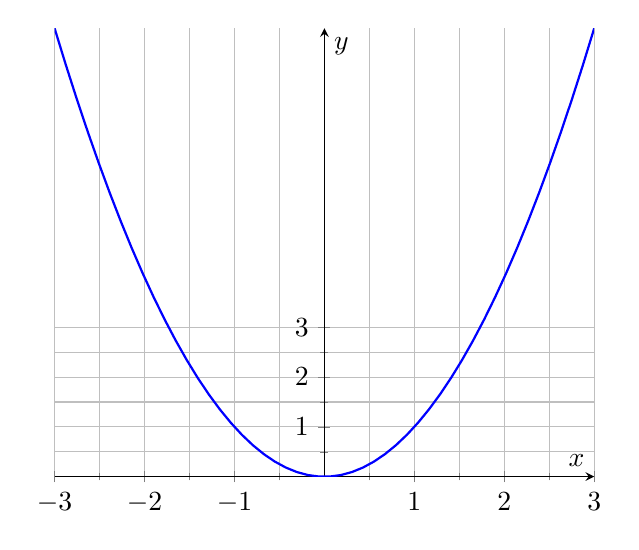
\begin{tikzpicture}
  \begin{axis}[
    axis lines=middle, % Draws x and y axes through the origin
    xlabel={$x$}, ylabel={$y$}, % Labels for clarity
    xtick={-3,-2,...,3}, % Explicit ticks on the x-axis
    ytick={-3,-2,...,3}, % Explicit ticks on the y-axis
    grid=both, % Adds a grid for reference
    minor tick num=1, % Adds minor ticks between major ones
  ]
    \addplot[domain=-3:3, samples=50, thick, blue]{x^2}; % Example curve
  \end{axis}
\end{tikzpicture}

